\section{Service Composition}

The main point of our investigation is a service-based environment where services are combined strategically with policies that cater to the specific needs of the user.
Our focus is on service composition, which involves three main actors and operates at a higher level of abstraction.
\begin{enumerate}
  \item The \User:
        The stakeholder within the service-based environment,
        the \user assumes the role of the entity initiating the request for a particular service.
        By choosing a template, the \user initiate the subsequent stages of the composition process.
  \item The Service Template:
        At the crux of effective service composition lies the pivotal role played by the service template.
        Functioning as a high-level composition of services labeled with predefined policies,
        the service template serves as a structured blueprint facilitating the decision-making process for the  \user.
        \begin{definition}[Service Template] \label{def:pipeline}
          A Service Template \T(\V,\E,$\iChartFunction{}$), is a direct acyclic graph having a root \vi{r}$\in$\V, a vertex \vi{i}$\in$\V\ for each service $s_i$,
          two additional vertices \vi{c},\vi{m}$\in$\V$_{\timesOperator}$$\subset$\V\ for each alternative ($\timesOperator$) structure modeling the alternative execution (\emph{choice}) of operations and the retrieval (\emph{merge}) of the results,
                respectively, and two additional vertices \vi{f},\vi{j}$\in$\V$_{\plusOperator}$$\subset$\V\ for each parallel ($\plusOperator$) structure modeling the contemporary execution (\emph{fork}) of operations and the integration (\emph{join}) of their results, respectively. $\iChartFunction{}$ is an annotation function, assigning to each vertex \vi{i}$\in$\V\ a set of policies \Pset{i}.
        \end{definition}
        % We note that $\{$\vi{r}$\}$ $\cup S_\timesOperator\cup S_\plusOperator=S$\\
  \item The Service Provider:
        Central to the execution of service composition is the service provider,
        serving as the responsible entity for delivering the requested service.
        Tasked with adhering to the prescribed service template, the service provider execute the service requested by the \user.
\end{enumerate}

% More detail about the structure modeling the alternative and parallel follows :

% \textbf{Sequence} ($\plusOperator$). It composes two service, $wsi$ and $wsj$, in a sequence. $wsi\plusOperator wsj$ mimics a composition where $wsj$ is executed after $wsi$.

% \textbf{Alternative} ($\timesOperator$). It composes two service, $wsi$ and $wsj$, in an alternative. $wsi\timesOperator wsj$ mimics a composition where either $wsi$ or $wsj$ is executed.

% \textbf{Parallel} ($\plusOperator$). It composes two service, $wsi$ and $wsj$, in parallel. $wsi\plusOperator wsj$ mimics a composition where both $wsi$ and $wsj$ are executed simultaneously.
\begin{figure}[h!]
  \centering
  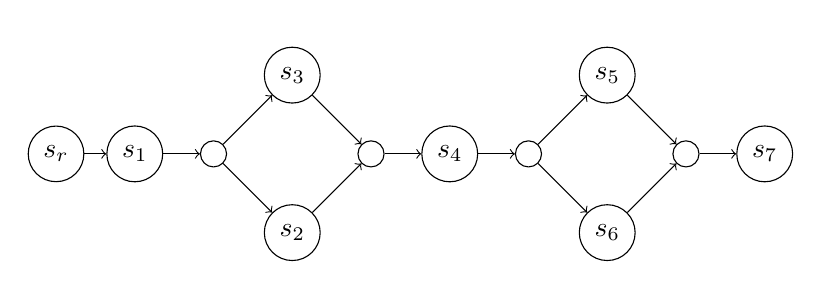
\begin{tikzpicture}
    % Nodes
    \node[draw, circle] (node1) at (0,0) {$s_r$};
    \node[draw, circle] (node2) at (1,0) {$s_1$};
    \node[draw, circle] (node3) at (2,0) {$\timesOperator$};
    \node[draw, circle] (node4) at (3,-1) {$s_2$};
    \node[draw, circle] (node5) at (3,1) {$s_3$};
    \node[draw, circle] (node6) at (4,0) {$\timesOperator$};
    \node[draw, circle] (node65) at (5,0) {$s_4$};
    \node[draw, circle] (node7) at (6,0) {$\plusOperator$};
    \node[draw, circle] (node8) at (7,1) {$s_5$};
    \node[draw, circle] (node9) at (7,-1) {$s_6$};
    \node[draw, circle] (node10) at (8,0) {$\plusOperator$};
    \node[draw, circle] (node11) at (9,0) {$s_7$};
    % Text on top
    \node[above] at (node1.north)  {$\tChartFunction$};
    \node[above] at (node2.north)  {$\tChartFunction$};
    \node[above] at (node3.north)  {                 };
    \node[above] at (node4.north)  {$\tChartFunction$};
    \node[above] at (node5.north)  {$\tChartFunction$};
    \node[above] at (node65.north) {$\tChartFunction$};
    \node[above] at (node8.north)  {$\tChartFunction$};
    \node[above] at (node9.north)  {$\tChartFunction$};
    \node[above] at (node11.north) {$\tChartFunction$};
    % Connection
    \draw[->] (node1) -- (node2);
    \draw[->] (node2) -- (node3);
    \draw[->] (node3) -- (node4);
    \draw[->] (node3) -- (node5);
    \draw[->] (node5) -- (node6);
    \draw[->] (node4) -- (node6);
    \draw[->] (node6) -- (node65);
    \draw[->] (node65) -- (node7);
    \draw[->] (node7) -- (node8);
    \draw[->] (node7) -- (node9);
    \draw[->] (node8) -- (node10);
    \draw[->] (node9) -- (node10);
    \draw[->] (node10) -- (node11);
  \end{tikzpicture}
  \caption{Service composition template}
  \label{fig:service_composition_template}
\end{figure}

\begin{figure}[h!]
  \centering
  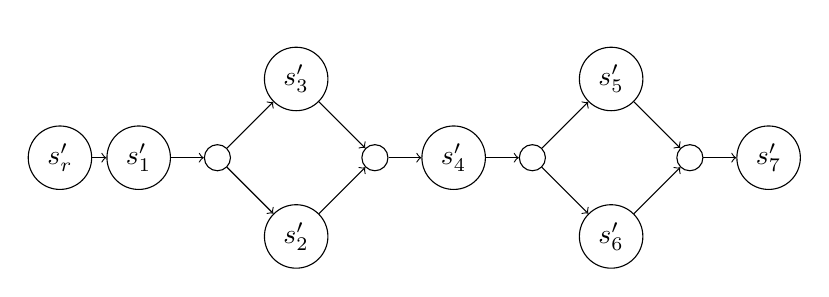
\begin{tikzpicture}
    % Nodes
    \node[draw, circle] (node1) at (0,0) {$s^\prime_r$};
    \node[draw, circle] (node2) at (1,0) {$s^\prime_1$};
    \node[draw, circle] (node3) at (2,0) {$\timesOperator$};
    \node[draw, circle] (node4) at (3,-1) {$s^\prime_2$};
    \node[draw, circle] (node5) at (3,1) {$s^\prime_3$};
    \node[draw, circle] (node6) at (4,0) {$\timesOperator$};
    \node[draw, circle] (node65) at (5,0) {$s^\prime_4$};
    \node[draw, circle] (node7) at (6,0) {$\plusOperator$};
    \node[draw, circle] (node8) at (7,1) {$s^\prime_5$};
    \node[draw, circle] (node9) at (7,-1) {$s^\prime_6$};
    \node[draw, circle] (node10) at (8,0) {$\plusOperator$};
    \node[draw, circle] (node11) at (9,0) {$s^\prime_7$};
    % Text on top
    \node[above] at (node1.north) { $\iChartFunction$};
    \node[above] at (node2.north) { $\iChartFunction$};
    \node[above] at (node3.north) {};
    \node[above] at (node4.north) { $\iChartFunction$};
    \node[above] at (node5.north) { $\iChartFunction$};
    \node[above] at (node65.north) { $\iChartFunction$};
    \node[above] at (node8.north) { $\iChartFunction$};
    \node[above] at (node9.north) { $\iChartFunction$};
    \node[above] at (node11.north) { $\iChartFunction$};
    % Connection
    \draw[->] (node1) -- (node2);
    \draw[->] (node2) -- (node3);
    \draw[->] (node3) -- (node4);
    \draw[->] (node3) -- (node5);
    \draw[->] (node5) -- (node6);
    \draw[->] (node4) -- (node6);
    \draw[->] (node6) -- (node65);
    \draw[->] (node65) -- (node7);
    \draw[->] (node7) -- (node8);
    \draw[->] (node7) -- (node9);
    \draw[->] (node8) -- (node10);
    \draw[->] (node9) -- (node10);
    \draw[->] (node10) -- (node11);
  \end{tikzpicture}
  \caption{Service composition instance}
  \label{fig:service_composition_instance}
\end{figure}




% \textbf{Loop} ($\oslash$). It composes a service composition by iteratively executing the same composition. $\oslash wsi$ mimics a composition where the service $wsi$ is executed a given number of times. In the following, $\oslash$ is considered as a sequence of $\oslash$ services with the same composition $wsi$.

% \textbf{Containment} ($\tau$). It composes two service, $wsi$ and $wsj$, in a containment relation. $wsi\tau wsj$ mimics a basic composition pattern where $wsj$ is called within $wsi$, meaning that $wsi$ assumes the role of a container and $wsj$ uses container-level functionalities (e.g., signature, encryption) to secure the message exchange. We note that the containment operator does not have a direct mapping to BPEL constructs because it is applied to a specific service before the BPEL process is even considered.
\subsection{Instance}
When the template is filled with the necessary services, it becomes an instance that reflects the actual implementation of those services. This instance follows the same flow as the template, but with the added function F that represents the transformation operations carried out by the service.

Let \T(\V,\E,$\iChartFunction$) be a Service Template, a Composite Service instance is \T'(\V',\E,$\iChartFunction$,$\gamma$) is a directed acyclic graph where:
$s_r=s'_r$, for each vertex \vi{}$\in$\V$_{\timesOperator}$$\cup$\V$_{\plusOperator}$ it exists a corresponding vertex \vi{}'$\in$\V'$_{\timesOperator}$$\cup$\V'$_{\plusOperator}$,
    and for each \vi{i}$\in$ \V\ it exists a corresponding \vi'{i}$\in$ \V'\ instantiated with a real service \vi{i} having a policy \Pset{i}, such that the following conditions hold:
    \begin{itemize}
      \item $s_i$ satisfies functional requirements in $G_{\iChartFunction}(V,E,\iChartFunction)$.
      \item \Pset{i} satisfies $\iChartFunction(v_i)$.
    \end{itemize}

    The Composite Service  instance  is generated by traversing the Service Template with a breadth-first search algorithm,
    starting from the root vertex \vi{r}. Then for each vertex \vi{i} in the Service Template, the corresponding vertex \vi{i}'$\in$ \V'\ is generated.
    Finally for each vertex  \vi{i}'$\in$ \V'\ a two step selection approach is applied as follows.
\begin{itemize}
  \item \textit{Selection Algorithm} - It matches requirements in $\iChartFunction(v_i)$ with the policy $\iChartFunction_i$, and returns a set of services $S_i$ that satisfy the requirements.
  \item \textit{Comparison Algorithm} - Upon retrieving a set of compatible services, it produces a ranking of these services according their scoring function.
        The scoring function is calculated according some metrics, which evaluate the quality of the data resulting from the service execution.
        More details about the metrics are provided in Section \ref{sec:metrics}.
\end{itemize}


\begin{figure}[H]
  \centering

  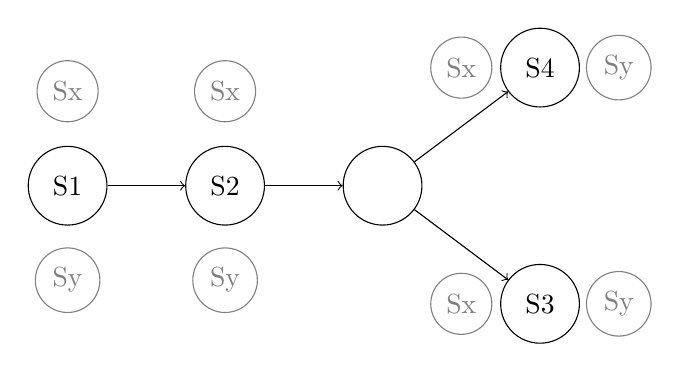
\begin{tikzpicture}
    % Nodes
    \node[draw, circle, minimum size=0.4cm, draw=gray, text opacity=0.5] (node11) at (0,1.2) {Sx};
    \node[draw, circle, minimum size=1cm] (node1) at (0,0) {S1};
    \node[draw, circle, minimum size=0.4cm, draw=gray, text opacity=0.5] (node10) at (0,-1.2) {Sy};

    \node[draw, circle, minimum size=0.4cm, draw=gray, text opacity=0.5] (node22) at (2,1.2) {Sx};
    \node[draw, circle, minimum size=1cm] (node2) at (2,0) {S2};
    \node[draw, circle, minimum size=0.4cm, draw=gray, text opacity=0.5] (node21) at (2,-1.2) {Sy};

    \node[draw, circle, minimum size=1cm] (node3) at (4,0) {$\timesOperator$};

    \node[draw, circle, minimum size=0.4cm, draw=gray, text opacity=0.5] (node42) at (5,-1.5) {Sx};
    \node[draw, circle, minimum size=1cm] (node4) at (6,-1.5) {S3};
    \node[draw, circle, minimum size=0.4cm, draw=gray, text opacity=0.5] (node41) at (7,-1.5) {Sy};

    \node[draw, circle, minimum size=1cm] (node5) at (6,1.5) {S4};
    \node[draw, circle, minimum size=0.4cm, draw=gray, text opacity=0.5] (node51) at (5,1.5) {Sx};
    \node[draw, circle, minimum size=0.4cm, draw=gray, text opacity=0.5] (node52) at (7,1.5) {Sy};
    % Connection
    \draw[->] (node1) -- (node2);
    \draw[->] (node2) -- (node3);
    \draw[->] (node3) -- (node4);
    \draw[->] (node3) -- (node5);
  \end{tikzpicture}
  \caption{Service composition instance}
  \label{fig:service_composition_instance}
\end{figure}
\[ \forall S \in \mathrm{S}_{C}  \exists  \iChartFunction(S) = \mathrm{S}_{1} \]


\begin{figure}
  \centering
  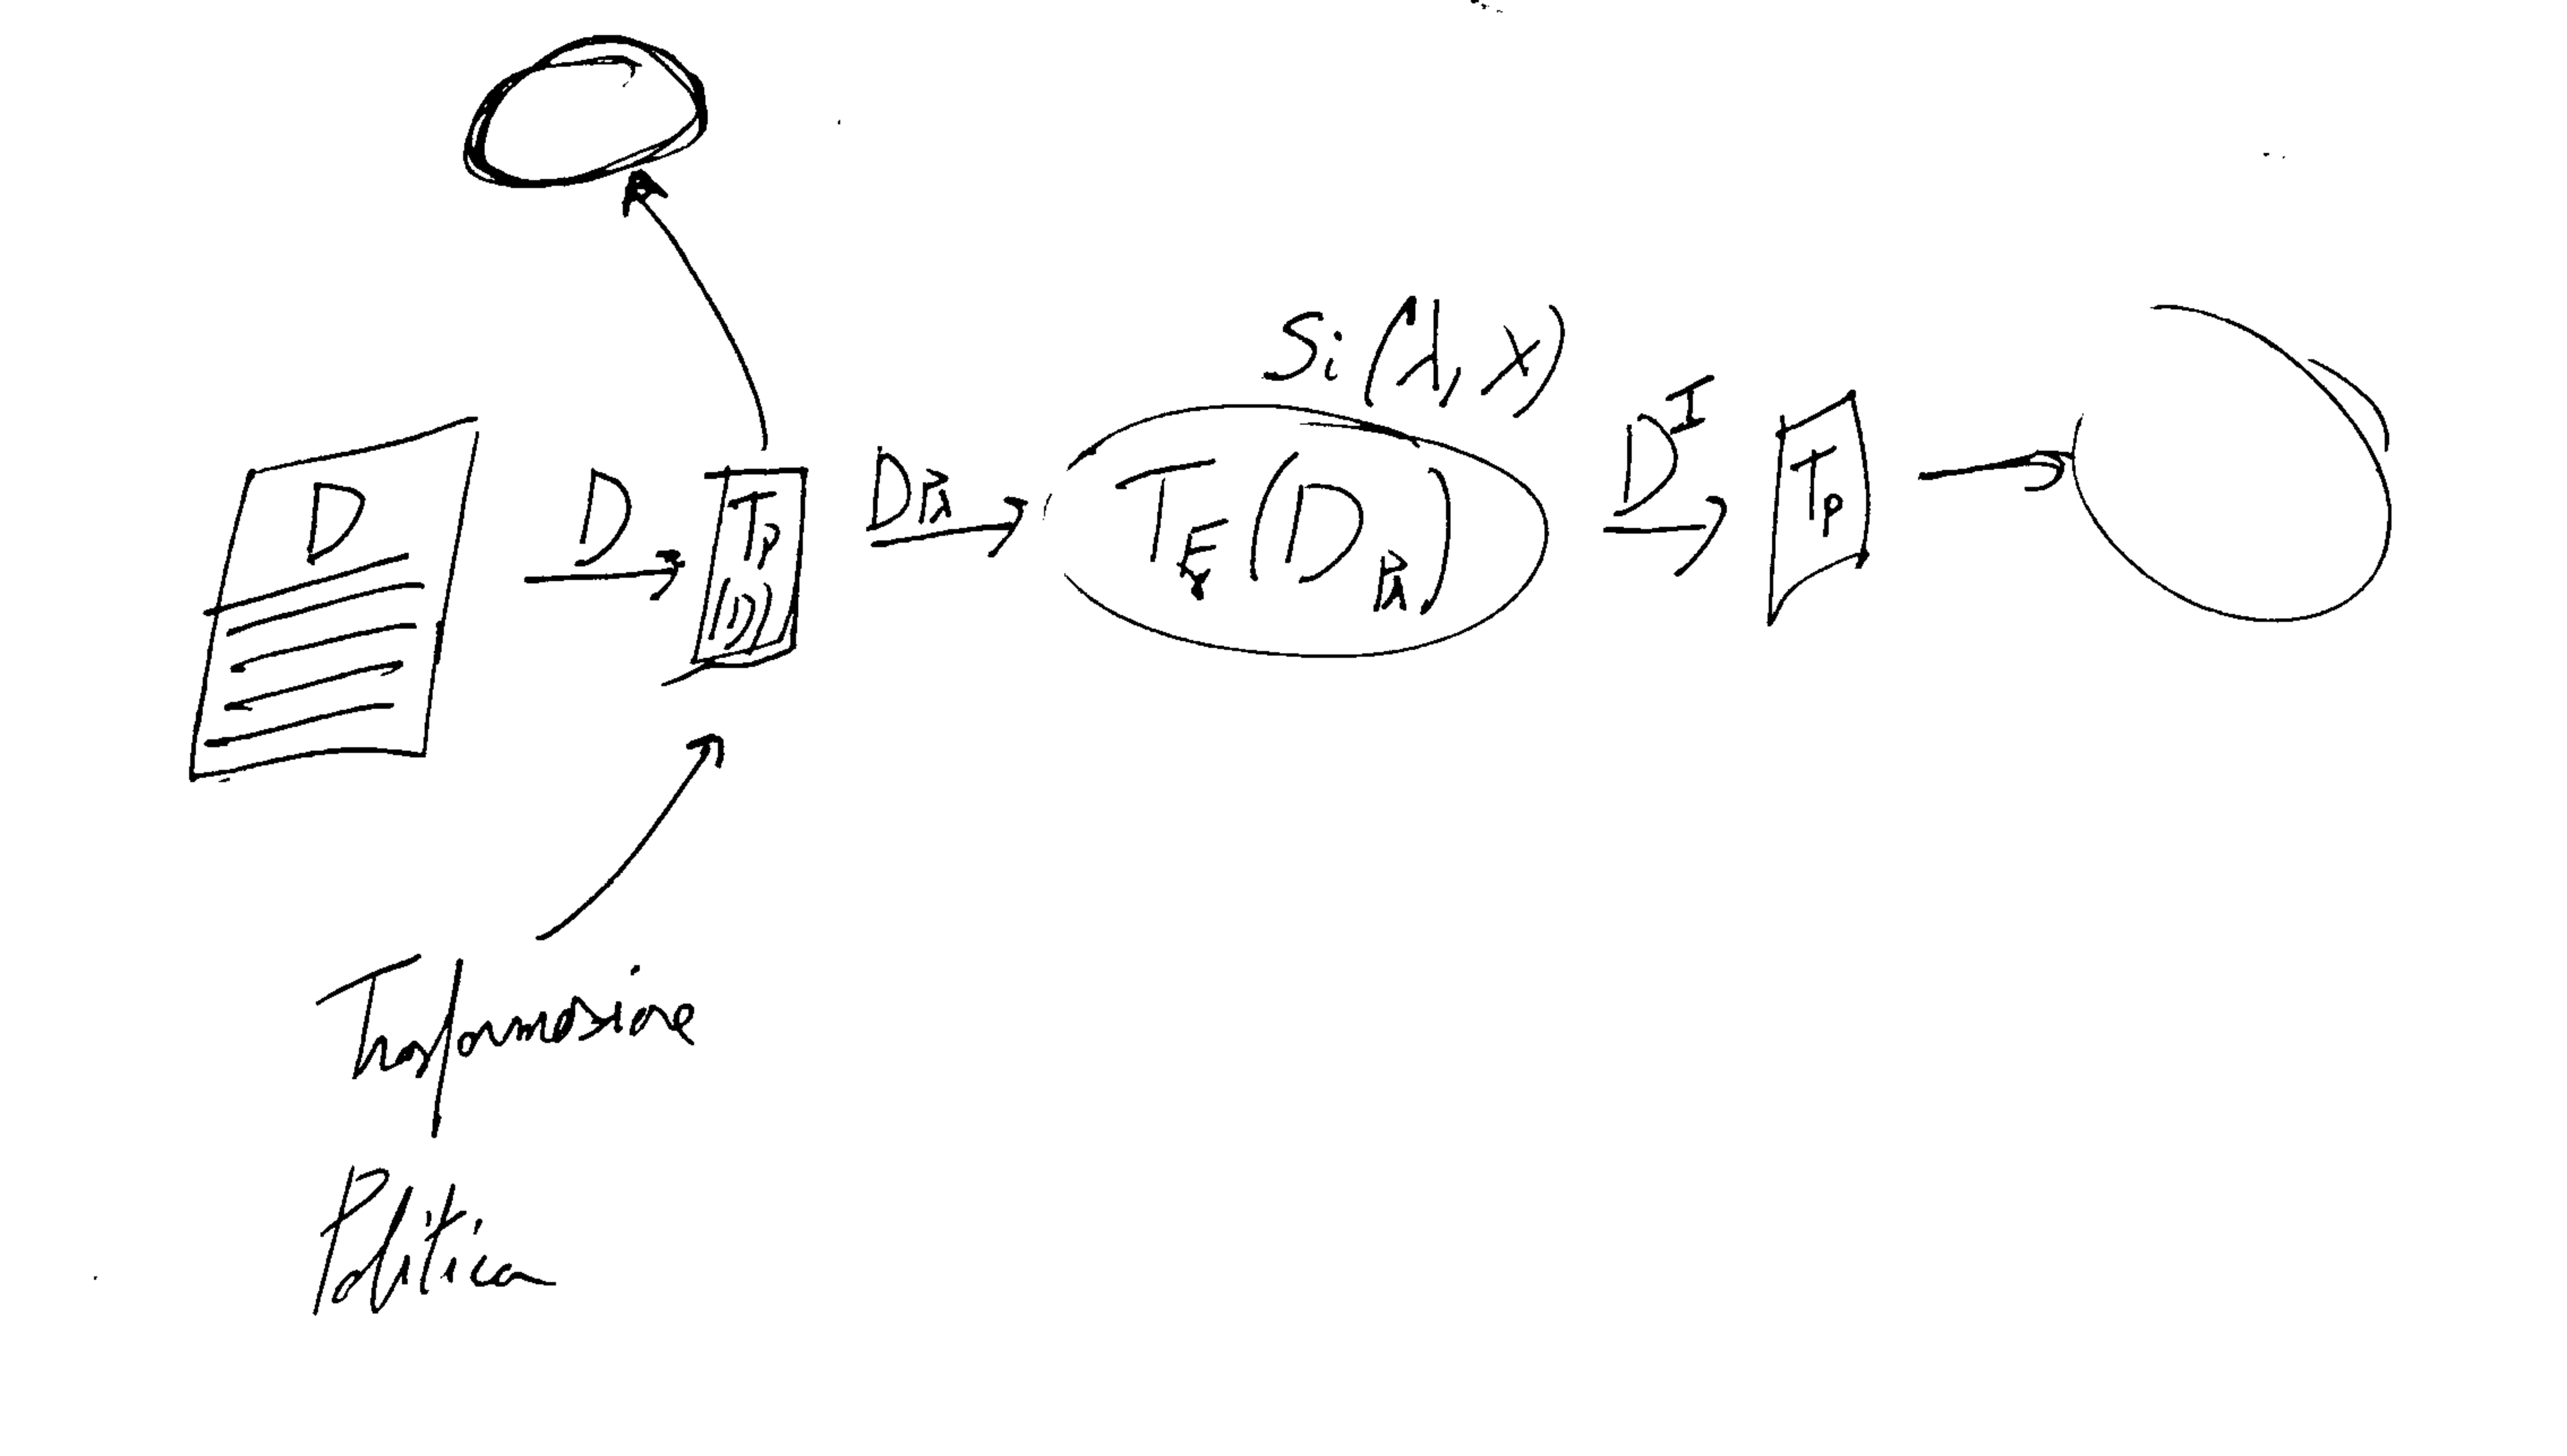
\includegraphics[width=\columnwidth]{serviceDetail.pdf}
  \caption{Service Detail}
  \label{fig:service_detail}
\end{figure}